\documentclass[
oneside,      % ← no paired (left-right) pages  
openany       % ← allow chapters to start on either side
]{imc-inf}

\title{3D Modeling of Microscopic Structures for Synthetic Data Generation Applications in AI Model Training for Microscopy Data}
\subtitle{\mbox{}} % if I leave it empty it throws an error
\thesistype{Bachelor Expos\'e}
\author{Alexander Savov}
\supervisor{Himanshu Buckchash} % what titles?
\copyrightyear{2025}
\submissiondate{2026.05.2025}
\keywords {Data Analytics, Machine Learning, Useability, Synthetic Data Generation, Microscopy, 3D Modeling, Deep Learning, Image Segmentation, Generative Models} % add keywords here 



% \usepackage{xyz}
\usepackage{listings}
\usepackage{subcaption}
\usepackage{placeins}


\begin{document}
	\frontmatter\maketitle{}
	
	\begin{declarations}\end{declarations}
	
	
	\begin{abstract}
		Microscopy plays a vital role in biomedical research and diagnostics, but training advanced AI models for microscopy image analysis requires abundant annotated image data. Obtaining high-quality labeled microscopy datasets is challenging due to labor-intensive manual annotation, expert subjectivity, and scarcity of rare or abnormal cases. This exposé proposes a novel pipeline for 3D modeling of microscopic structures to generate realistic synthetic microscopy images for training AI models. The goal is to alleviate the data bottleneck by producing physics-informed synthetic data that closely mimics real microscope images, thereby improving model robustness and accuracy. The planned pipeline will parametrically model subcellular structures in 3D (e.g. using geometric primitives to represent organelles), render them into 2D images with simulated microscope optics and noise, and create large annotated datasets without manual labeling. We will investigate generative strategies (simulation-based and AI-driven) to maximize the realism of synthetic images and examine how using 3D synthetic data in model training impacts performance. We hypothesize that augmenting or pre-training with synthetic data will lead to more robust models, able to generalize better to new microscopic images. The exposé outlines the relevant background, research questions, proposed methodology including an evaluation plan with quantitative metrics (image similarity and model accuracy), expected outcomes, and a work plan. This work will lay the foundation for a bachelor thesis aimed at demonstrating that 3D synthetic microscopy data can enhance deep learning models for microscopic image analysis while reducing reliance on scarce hand-annotated samples.
		
	\end{abstract}
	
	
	%\begin{acknowledgements} % I dont have anything here YET !!!!!!!!!!!!!!!!!!!!!!!!!!!
	%This is an \textbf{optional} page. Use your choice of paragraph style for text on this page. Usually, this %space is for thanking your supporters and getting emotional about how grateful you are to everyone.  
	%\end{acknowledgements}
	
	\addtoToC{Table of Contents}% this gets generated titles used
	\tableofcontents%
	\clearpage
	
	\addtoToC{List of Figures}%
	\listoffigures         
	\clearpage
	
	
	%   MAIN MATTER  %%%%%%%%%%%%%%%%%%%%%%%%%%%%%%%%%%%%%%%%%%%%%%%%%%%%%%%%%%%%%%
	\mainmatter%
	
	\chapter{Introduction}\label{chap:introduction}
	
	Advances in microscopy techniques are producing vast amounts of high-resolution imagery of cells and tissues. These images hold rich information for biomedical research, such as understanding cell morphology, tracking subcellular dynamics, and identifying pathological changes. In recent years, artificial intelligence (AI) and deep learning models have demonstrated remarkable success in analyzing microscope images, enabling tasks like cell segmentation, object tracking, and phenotypic classification~\cite{ronneberger2015unet,lecun2015deep}.
	
	However, training deep learning models reliably for microscopy data remains challenging due to the scarcity of annotated training data. Preparing ground truth annotations for microscopic structures is a tedious and expertise-dependent process: biologists must manually delineate or label tiny organelles (often on the order of 100–1000 nm in size) in images that are noisy and blurred by optical limitations~\cite{sekh2021}. Manual segmentation is not only time-consuming (as shown by Sekh et al., who report that segmenting just 30 microscopy frames can take hours~\cite{sekh2021}), but also prone to inconsistency and subjectivity between annotators~\cite{litjens2017survey}. This leads to ground truth (GT) ambiguity for training AI models: the lack of clear, large-scale labeled datasets hinders supervised learning in this domain~\cite{litjens2017survey}.
	
	Conventional approaches to obtain training data—such as in vitro experiments with fluorescent markers and subsequent manual annotation or semi-automatic thresholding—are reaching their limits. Simple image processing (e.g., Otsu thresholding) often fails on subcellular structures due to noise and blur, yielding grossly inaccurate results~\cite{otsu1979threshold}. As a result, researchers have begun exploring simulation and synthetic data generation as alternative ways to produce training datasets. The central idea is to leverage computational modeling to create artificial microscope images where the true object labels are known a priori. This approach is sometimes called simulation-supervised learning, as it uses simulated images with perfect labels to train models~\cite{sekh2021}.
	
	Notably, Sekh et al. (2021) introduced a physics-based simulation pipeline to generate microscope images of mitochondria and vesicles, which provided unambiguous ground truth for training a segmentation network~\cite{sekh2021}. By using synthetic images rendered with realistic optical blur and noise, their deep learning model achieved improved accuracy and speed in subcellular segmentation compared to models trained on scarce manual annotations. This underscores the promising role of synthetic data in advancing microscopy AI.
	
	Despite these developments, important gaps remain. Many previous efforts in synthetic data for microscopy have focused on two-dimensional (2D) image simulation or augmenting existing images (e.g., applying transformations to real images). Less explored is the 3D modeling of microscopic structures with parametric flexibility – i.e., constructing 3D digital models of organelles or cells that can be systematically varied in shape and then projected to images. A physically-informed 3D modeling approach could capture structural variations (size, shape, spatial arrangement) more comprehensively than 2D augmentations. If successful, this would enable generation of diverse and realistic training images, including rare or extreme cases that are under-represented in real data.
	
	The goal of this exposé is to formulate how such a 3D synthetic data pipeline can be designed and how it will improve AI model training for microscopy. In the following, we review related work (Section~\ref{chap:related-work}), formalize the research questions (Section~\ref{chap:research-questions}), then detail the proposed methodology (Section~\ref{chap:methodology}) and evaluation plan (Section~\ref{chap:evaluation}). Expected outcomes and a project timeline are also presented (Sections~\ref{chap:expected-results} and~\ref{chap:timeline}). By addressing these points, the exposé lays the groundwork for a bachelor thesis that aims to demonstrate the value of 3D synthetic microscopy data in training robust AI models.
	
	
	\section{Background and Literature Review}\label{chap:related-work}
	
	\subsection{Data Challenges in Microscopy AI}
	\textbf{Data Challenges in Microscopy AI:}
	Deep learning models generally require large amounts of annotated data, yet in microscopy obtaining such annotations is notoriously difficult.
	Ronneberger \emph{et al.}\ documented that “successful training of deep networks requires many thousand annotated samples” for their U-Net architecture and the ISBI Cell-Tracking Challenge 2015~\cite{ronneberger2015unet}.
	Creating those thousands of pixel-accurate masks is often impractical in specialised domains (e.g.\ fluorescence images of sub-cellular organelles).
	Experts can spend hours per image and still produce inconsistent labels, leading to ground-truth ambiguity that hampers supervised learning~\cite{litjens2017survey}.
	This bottleneck has motivated researchers to look for alternative data sources such as physics-based simulation and generative models.
	
	\subsection{Synthetic Data Generation Approaches}
	\textbf{Synthetic Data Generation Approaches:}
	One remedy for data scarcity is the \textbf{in-silico} generation of image/label pairs.
	Sekh \emph{et al.}\ presented a physics-based pipeline that generates 3-D models of mitochondria or vesicles, applies an optical point-spread function, adds realistic noise, and outputs perfectly labelled fluorescence images~\cite{sekh2021}.
	Their simulation-supervised network achieved state-of-the-art accuracy on real EM data after fine-tuning.
	A similar idea was used by Punnakkal \emph{et al.}\ to quantify mitochondrial morphology purely from simulation-trained models~\cite{punnakkal2023}.
	Zhao \emph{et al.}\ pushed the concept further with \emph{Sarc-Graph}, voxelising parametric sarcomere models, projecting them to 2-D, and demonstrating that identical parameters segment both synthetic and real beating-cardiomyocyte videos~\cite{zhao2021}.
	These works illustrate the power of \textbf{physics-based synthetic data}: by encoding known imaging optics and biologically realistic shape variability, one can generate unlimited, perfectly labelled examples for training modern deep networks.
	
	
	\begin{figure}[ht] % this shit goes to a new line and lets some text pass for no reason
		\centering
		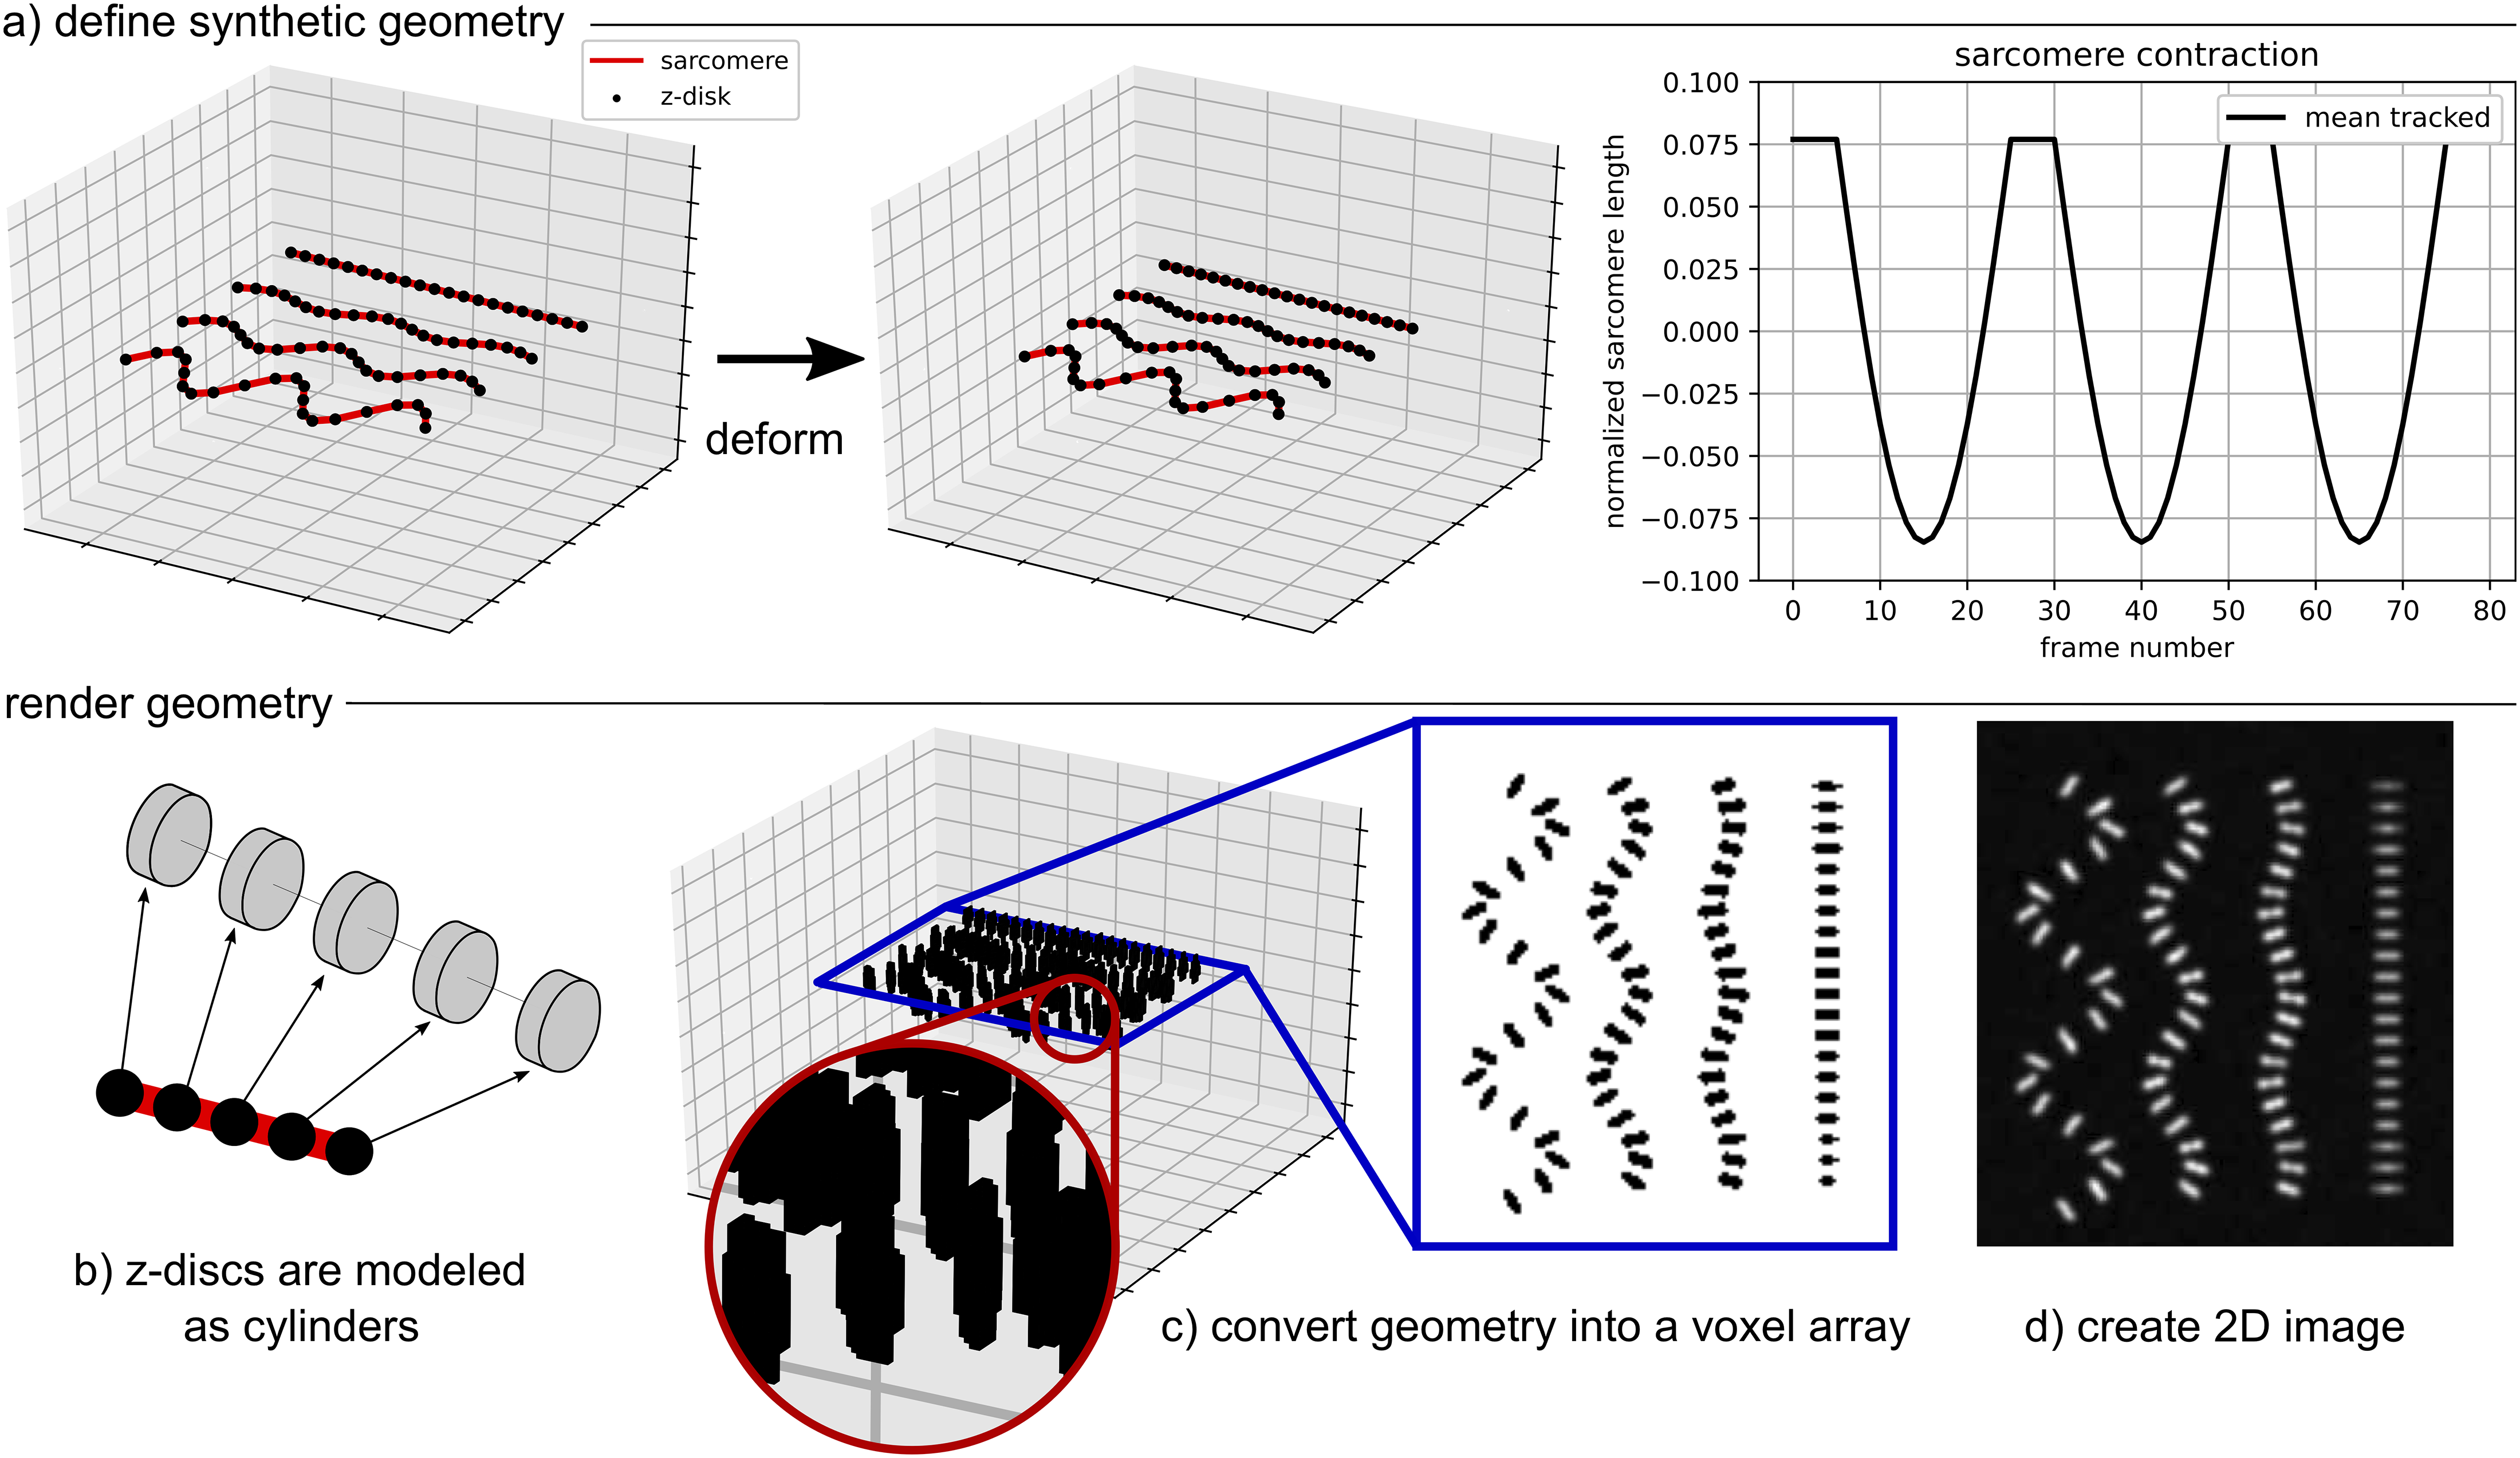
\includegraphics[width=1.0\textwidth]{journal.pcbi.1009443.g002.png}
		\caption{Example synthetic-data pipeline (adapted from Zhao \textit{et al.}\,\cite{zhao2021}).}
		\label{fig:logo}
	\end{figure}
	
	
	\FloatBarrier % ← This forces LaTeX to place the image before continuing 
	
	
	
	Starting with a 3-D geometric model of the structures of interest (e.g.\ points
	representing Z-discs and line segments for sarcomeres in a cardiomyocyte), the
	pipeline converts this model into a 3-D voxel representation and then into a
	2-D image slice.  Microscope blur and noise are added to produce a realistic
	synthetic fluorescence image.  The known 3-D geometry therefore serves as
	ground-truth for validating segmentation and tracking
	algorithms~\cite{zhao2021}.
	
	\medskip
	
	\textbf{Figure~\ref{fig:logo}}, adapted from Zhao~\textit{et al.}~\cite{zhao2021},
	illustrates a full synthetic-data pipeline for microscopy-analysis software.
	The pipeline first defines the \textbf{geometry} of the biological structure in
	3-D (points for sarcomere anchor points and connecting line segments) and even
	prescribes dynamic changes such as contraction over time.  Next, the geometric
	elements are given volumetric shape (each point is approximated by a small 3-D
	cylinder) and the scene is \textbf{voxelised} at anisotropic resolution
	(higher lateral than axial sampling).  A 2-D image slice is then obtained by
	projection, after which \textbf{optical blur and noise} are introduced: the
	voxel volume is convolved with a Gaussian point-spread function and Perlin /
	Poisson noise is added to mimic camera read-out.  The resulting synthetic
	images closely match real wide-field recordings, yet all object identities are
	known.  Zhao~\textit{et al.} showed that their Sarc-Graph software could
	segment and track sarcomeres equally well on synthetic and real videos without
	extra parameter tuning, demonstrating that \textbf{investment in high-fidelity
		synthetic data pays off}~\cite{zhao2021}.
	
	\medskip
	Beyond physics-based simulation, researchers have explored \textbf{generative AI models}.  Majurski~\textit{et al.}~\cite{majurski2019gan} used a GAN, together with transfer learning, to synthesise realistic cell images and
	boost segmentation accuracy.  Diffusion models and other modern generators are now being tested for image-level augmentation in microscopy as well.  The key challenge with purely generative approaches is obtaining correct labels; one solution is to train conditional generators that output image/label pairs from a given segmentation mask.
	
	In summary, two complementary strategies exist for synthetic microscopy data: (i) forward physical simulation of image formation, which guarantees perfect	labels, and (ii) learning-based image generation, which can maximise visual	realism.  This exposé emphasises the former for label accuracy while using the latter as an optional refinement step to close any residual realism gap.
	
	
	\subsection{Microscopic Structure Modeling}
	
	\textbf{Microscopic Structure Modeling:} Modeling the shape of microscopic structures is a prerequisite for generating realistic synthetic images. There have been efforts to create computational models for cell and organelle morphology (e.g., Sbalzarini et al.’s work on cell shape modeling). Techniques range from simple geometric primitives (spheres, ellipsoids, cylinders to approximate nuclei, mitochondria, filaments, etc.) to more complex approaches like point process models or agent-based models that capture spatial organization. For example, FluoSim (Lagardère \textit{et al.}, 2020) simulates single-molecule microscopy by modeling molecules diffusing and binding in a geometrical cell membrane region \cite{lagardere2020fluosim}. TestSTORM (Novák \textit{et al.}, 2017) generates synthetic super-resolution microscopy images by simulating fluorophore blinking and localization errors in 3-D space \cite{novak2017teststorm}. These tools highlight the importance of accurate geometric and physical modeling: the more faithfully we capture the structure (and the imaging physics), the more the synthetic data will reflect true biological images. However, most existing simulators focus on specific imaging modalities or 2D projections. There is a need for flexible \textbf{3D modeling frameworks} where one can construct an organelle or cell in silico (potentially using parametric shapes or meshes) and render it under different imaging settings.
	
	In particular, mitochondria are often cited as an example of morphologically complex organelles. They form networks of tubules that constantly change shape. An analysis by Punnakkal et al. (2023) used a physics-based learning tool to segment mitochondria in 2D images and quantify their shape features \cite{punnakkal2023}. Their simulator was tailored to fixed-cell fluorescence images, and by training on those simulations, the model could detect morphological changes induced experimentally \cite{punnakkal2023}. This indicates that by capturing key shape variations (branch lengths, fragmentation, etc.) in the synthetic data, the trained model can be sensitive to real biological differences. Similarly, other structures like cell nuclei or actin filaments could be modeled with parametric shapes (e.g. random deformable ellipsoids for nuclei, spline curves for filament networks). The literature suggests that \textbf{parametric 3D modeling combined with domain-specific knowledge} (such as distribution of fluorescent markers, typical sizes) is a viable path to create synthetic images that meaningfully augment real data.
	
	\subsection{Impact of Synthetic Data on Model Performance}
	\textbf{Impact of Synthetic Data on Model Performance:} A crucial question is whether training on synthetic data actually improves model performance on real data. Early evidence is encouraging. Sekh \textit{et al.} reported that their simulation-trained network not only performed well on synthetic test images but also generalised to real microscopy images of the same structures—and could be transfer-learned to different microscopes—despite the absence of large ground-truth datasets \cite{sekh2021}. Zhang \textit{et al.} (2023) likewise showed that augmenting training with synthetic images enabled a deep model to rapidly detect neurons in calcium-imaging videos with high accuracy \cite{zhang2023synthetic}. Zhao \textit{et al.} (2021) validated their Sarc-Graph tool by comparing its output on synthetic videos (where ground truth was known) with the known labels, then demonstrated similar performance on real beating-cardiomyocyte videos without further parameter tuning \cite{zhao2021}. Networks trained with a mixture of physics-based simulations and GAN-generated images also tend to over-fit less to small real datasets and cope better with noise or rare events \cite{majurski2019gan}. Of course, the benefit depends on the fidelity of the synthetic images—if they miss important features, models can learn spurious patterns—so current research focuses on making simulations as realistic and representative as possible. Objective measures such as the \textbf{Structural Similarity Index (SSIM)} are often used to quantify realism by comparing synthetic to real images \cite{wang2004image}; values close to 1 indicate that the synthetic images are visually and statistically indistinguishable from their real counterparts.
	
	In summary, the literature shows a clear trend: \textbf{synthetic microscopy data generation is emerging as a key tool} to overcome data scarcity, with physics-based simulations ensuring label accuracy and generative models enhancing realism. A remaining gap is the lack of comprehensive 3-D modelling of biological structures; the present exposé therefore proposes a pipeline that uses parametric 3-D models to generate synthetic training data and systematically analyses how different generative strategies affect image realism and downstream model performance.
	
	
	
	
	\chapter{Research Questions}\label{chap:research-questions}
	
	Based on the above context, the exposé will address the following research questions (RQs):
	
	\section{What are the methods to design and implement a 3D synthetic-data pipeline for training AI models in microscopy?}
	
	\textbf{RQ1:} This question focuses on the engineering and design of the pipeline: how to create 3D models of microscopic structures, how to simulate the imaging process (optics and noise), and how to efficiently generate labeled datasets. It involves exploring tools and methods from computer graphics and computational microscopy to build an end-to-end pipeline.
	
	\section{Which generative modeling strategies support producing better realistic synthetic microscopy images for AI-based analysis?}
	
	\textbf{RQ2:} Here we compare strategies for synthetic image generation: for example, physics-based rendering vs. deep generative models (GANs, etc.). “Better realistic” implies we will evaluate image realism and how closely synthetic images approximate real microscope images. The goal is to determine which approach (or combination) yields synthetic data that leads to optimal AI model performance.
	
	\section{To what extent does 3D synthetic data improve the robustness and accuracy of AI models for microscopic image analysis?}
	
	\textbf{RQ3:} This question evaluates the impact of using synthetic data in training. We will quantify improvements in model robustness (ability to handle variations and noise) and accuracy on real-world tasks when the model is trained or augmented with 3D synthetic data. Essentially, we ask: how big is the benefit of synthetic data, and in what ways (e.g., higher validation accuracy, better generalization to new datasets, reduced error on edge cases)?
	
	\vspace{1.5em} % so that is is not glued to the top part
	Each question corresponds to a key aspect of the thesis: RQ1 addresses the implementation of the solution, RQ2 addresses the quality of synthetic data, and RQ3 addresses the outcome on AI model performance. Together, they will guide the research and development in the subsequent thesis work.
	
	
	
	\chapter{Methodology}\label{chap:methodology}
	To answer the research questions, a structured methodology is proposed, consisting of: (1) \textbf{Designing a 3D synthetic data generation pipeline} (addressing RQ1), (2) \textbf{Implementing and testing different generative strategies for realism} (addressing RQ2), and (3) \textbf{Training and evaluating AI models with synthetic data} (addressing RQ3). We detail each component below.
	
	\section{Synthetic Data Generation Pipeline}
	The first step is to develop a pipeline that can generate synthetic microscopy images with corresponding ground truth labels. The pipeline will be built in a modular fashion, with stages reflecting the actual image formation process:
	
	\begin{itemize}
		\item \textbf{3D Structure Modeling:} We will create parameterized 3D models of the microscopic structures of interest. For example, if focusing on mitochondria (as a running case study), we can represent them as 3D tubular networks. Simpler organelles like cell nuclei could be modeled as ellipsoids, and linear structures like actin filaments as spline curves or cylinders. The modeling will leverage libraries such as \emph{Trimesh} or \emph{Open3D} for constructing and manipulating meshes. Key parameters (which can be randomized) include size (length, diameter), shape complexity (branching, bending of tubules), and spatial distribution (how many objects, how they are arranged in a volume). This addresses \textbf{RQ1} by establishing \emph{methods to represent microscopic geometries}. Prior works inform this stage: Sekh \emph{et al.} computed a triangulated surface for each mitochondrion based on expected size~\cite{sekh2021}, while Zhao \emph{et al.} used points and lines to represent sarcomeres and then gave them thickness by cylinders~\cite{zhao2021}. Our pipeline will generalize these ideas to whatever structure we target, providing a flexible parametric model that can generate a variety of shapes.
		
		\item \textbf{Fluorophore / Intensity Simulation:}	In fluorescence microscopy, the brightness of structures depends on fluorescent markers. We will simulate the distribution of fluorescent molecules (fluorophores) within the 3-D model. For instance, for a volumetric structure, we might randomly distribute points inside it representing fluorescent emitters (with density corresponding to staining intensity). Alternatively, we can assign an intensity function to the mesh (e.g., uniform or gradient). Sekh \textit{et al.}\ included photokinetics of fluorescent molecules in their simulation to model blinking or bleaching \cite{sekh2021}, but for our initial pipeline we may assume static intensity. The output of this step is a 3-D grid of intensities (a voxel volume) representing the ground-truth fluorescent signal prior to imaging.	This naturally yields a \textbf{ground-truth segmentation mask} as	well, by thresholding the voxel volume to 1 wherever structure is	present (similar to the physics-based GT method that projects and binarises the known locations of fluorophores \cite{sekh2021}). Generating this mask is straightforward since we know the exact geometry.
		
		\item \textbf{Optical Imaging Simulation:} Next, the pipeline will simulate the imaging process of a microscope. We will incorporate a 3-D point-spread function (PSF) corresponding to the microscope’s optics. The PSF describes how a point source of light appears blurred in the image; in 3-D it typically has a lobed ellipsoidal shape. We can use a theoretical PSF (e.g., a Gaussian approximation or Gibson–Lanni model for wide-field microscopy) or even an experimentally measured PSF if available. The 3-D fluorescent-intensity volume from the previous step will be convolved with the PSF, which blurs the signal in \(x,y,z\), mimicking the finite resolution and out-of-focus effects \cite{sekh2021}. After applying the PSF, we obtain a simulated raw image volume. In many microscope modalities (such as confocal or wide-field), a camera captures a 2-D projection of the 3-D volume. We will simulate this by slicing or projecting the volume to a 2-D plane. For wide-field microscopy, a reasonable approximation is to take a thin slice (or a maximum-intensity projection) around the focal plane \cite{zhao2021}. The Sarc-Graph pipeline in PLOS Computational Biology explicitly slices and projects the voxel array to get the final 2-D image \cite{zhao2021}, which we will emulate. The result is a 2-D image where our structures appear with realistic blur and intensity profiles, as if imaged under a microscope.
		
		\item \textbf{Noise Addition:} Real microscopy images contain various sources of noise: photon shot noise (Poisson-distributed, due to the discrete nature of light), electronic read noise (often approximated as Gaussian), and background autofluorescence. To ensure synthetic images are \textbf{indistinguishable from real} in noise characteristics, we will add noise to the 2-D images. A simplified but effective approach is to add Poisson noise based on photon counts (we can scale our image to a certain photon-count level and random-sample), followed by Gaussian noise to simulate camera read noise \cite{zhao2021}. We may also consider spatially correlated noise such as speckles; Zhao \textit{et al.}\ added Perlin noise for a textured background \cite{zhao2021}. By tuning noise parameters (variance, etc.) to match typical signal-to-noise ratios observed in real images—which can be as low as $\mathrm{SNR}\approx2\!-\!4$ in challenging live-cell conditions \cite{sekh2021}—we will strive for high realism. Image realism will be validated by comparing histograms and intensity distributions between synthetic and sample real images.
		
	\end{itemize}
	
	By the end of this pipeline, we will have: (a) synthetic microscope images, and (b) ground truth masks for the structures in those images (derived from the known 3D models). This addresses RQ1, as it provides a concrete implementation of a 3D synthetic-data pipeline.
	To facilitate large dataset generation, the pipeline will be scripted to produce many variants. We will randomize parameters for each generated image: e.g., one image might contain a few large mitochondria, another many small fragmented ones; different noise realizations will be applied; the focal plane can be varied. Thousands of images can be generated relatively quickly once the pipeline is implemented (the slowest step is likely the PSF convolution, but that can be accelerated via FFT or GPU). We plan to generate on the order of 5,000–10,000 synthetic images for the training dataset, as suggested in the project outline. This number is chosen to be sufficiently large to train deep networks, yet manageable in terms of storage and generation time.
	To explore RQ2 (realism strategies), we will implement two modes in the pipeline:
	•	A pure simulation mode as described above (hand-crafted, physics-based).
	•	A GAN-based enhancement mode: here, we would take the output of our physics simulation (which may be slightly idealized) and feed it through a trained generative model to improve realism. For instance, we could train a CycleGAN or similar network that takes a “clean” simulated image and outputs a more “realistic” image by learning from unpaired real data. Alternatively, we might use style transfer to match the texture of real microscopy images. This hybrid approach has been used in some contexts to refine simulations (often termed Sim2Real translation).
	Comparing these modes will inform RQ2: if GAN-enhanced images lead to better model performance (or higher realism metrics) than the raw physics simulation, that indicates the generative model is adding value. If not, it might mean the physics-based images were already sufficient or that the GAN introduced artifacts.
	
	\vspace{1.5em}
	To explore \textbf{RQ2} (realism strategies), we will implement two modes in the pipeline:
	
	\begin{itemize}
		\item A \textbf{pure simulation mode} as described above (hand-crafted, physics-based).
		
		\item A \textbf{GAN-based enhancement} mode: here, we would take the output of our physics simulation (which may be slightly idealized) and feed it through a trained generative model to improve realism. For instance, we could train a CycleGAN or similar network that takes a “clean” simulated image and outputs a more “realistic” image by learning from unpaired real data. Alternatively, we might use style transfer to match the texture of real microscopy images. This hybrid approach has been used in some contexts to refine simulations (often termed Sim2Real translation).
	\end{itemize}
	
	Comparing these modes will inform RQ2: if GAN-enhanced images lead to better model performance (or higher realism metrics) than the raw physics simulation, that indicates the generative model is adding value. If not, it might mean the physics-based images were already sufficient or that the GAN introduced artifacts
	
	\section{AI Model Training Strategy}
	With the synthetic data in hand, the next part of the methodology is to train AI models and evaluate the impact of synthetic data on their performance. This directly addresses RQ3. Our plan is to set up several experimental conditions:
	
	
	\begin{itemize} % PROBLEM: the first proper citation and it is [?]
		
		\item \textbf{Model Architecture:} We will likely use a U-Net CNN architecture (or a close variant) for segmentation tasks, given its popularity and success in microscopy~\cite{ronneberger2015unet}. U-Net is well-suited for our experiments as it can segment images pixel-by-pixel and is robust to limited data through its augmentation strategy. We may also explore other architectures or tasks; for example, a ResNet classifier if the task was classification. But segmentation of structures seems a fitting task for evaluating morphological accuracy and is aligned with the nature of our synthetic data (which comes with segmentation masks).
		
		\item \textbf{Training Datasets:} We will train the model under three scenarios: (1) using real microscopy data only, (2) using synthetic data only, and (3) using a hybrid mix of real + synthetic. For scenario (1), we will collect a small real dataset. Given the difficulty of manual labeling, we expect this real set to be limited (perhaps on the order of tens of images with annotations, which is typical in biomedical segmentation challenges). Scenario (2) will use the large synthetic dataset generated by our pipeline, with perfect labels. Scenario (3) will combine both: for instance, starting training on synthetic and fine-tuning on real, or simply pooling datasets (depending on what yields better results). The strategy of pre-training on synthetic then fine-tuning on a small real dataset is appealing, as it can leverage the advantages of both – the breadth of synthetic data and the authenticity of real data for final adjustments \cite{zhang2023synthetic}. We will experiment with both pooling and sequential fine-tuning approaches.
		
		\item \textbf{Training Protocol:} All models will be trained with the same hyperparameters as much as possible (learning rate, epochs, etc.) to ensure fairness. Data augmentation (like random flips, rotations) will be applied in all cases to avoid any bias (though the synthetic set already comes with a lot of random variations by design). We will monitor training and validation loss, and use early stopping or model checkpointing to avoid overfitting. In the case of synthetic-only training, overfitting is less a concern due to the large dataset, but we must be wary of simulator bias – the model might overfit to features of synthetic images that don’t translate to real images. This is where scenario (3) is critical, as it can help the model adjust to real image characteristics.
		
		\item \textbf{Baseline Comparison:} If feasible, we will also compare against a simpler baseline model or method. For example, a classical image-processing approach—such as Otsu thresholding—can be evaluated on the real test data to show how a learning-based approach improves upon it \cite{otsu1979threshold}. Additionally, if any pre-trained networks on similar data exist (perhaps models from the Cell Tracking Challenge or others), we could include them for reference. The primary baseline, however, will be real-only training, as this represents the conventional scenario. Our expectation is that incorporating synthetic data will outperform this baseline.
		
		
	\end{itemize}
	
	After training, the evaluation procedure (details in the next section) will compare the outcomes of these scenarios to answer RQ3. Essentially, we will look at metrics on a hold-out test set of real microscope images (which were not seen in training by any of the models) to see which training scenario yields the best performance. We anticipate that the hybrid (real + synthetic) training will perform the best, as suggested by prior studies that saw improvements when using synthetic data\cite{zhang2023synthetic}. Synthetic-only training might perform well too, but possibly slightly below hybrid if there is some residual domain gap. Real-only is likely to underperform due to the small training sample size.
	To support RQ2 in the context of training, we will also compare if models trained on more realistic synthetic data (e.g., after a GAN-based refinement) have better test performance than those trained on the initial pipeline output. This will tell us if investing in advanced generative modeling yields tangible gains in model accuracy.
	Throughout this methodology, careful documentation and versioning will be maintained (e.g., keeping track of dataset parameters, random seeds for reproducibility, and training logs). This ensures that results can be attributed to changes in data generation or training strategy.
	
	
	
	
	\chapter{Evaluation Plan}\label{chap:evaluation}
	A comprehensive evaluation plan is essential to quantitatively measure: (a) the realism of synthetic data (RQ2), and (b) the performance and robustness of models trained with synthetic data (RQ3). The evaluation will consist of the following components:
	
	\section{Image Realism Evaluation}
	\textbf{1. Image Realism Evaluation:} To address RQ2, we will assess how close the synthetic images are to real microscopy images. We will use quantitative metrics and visual inspections:
	
	
	\begin{itemize}
		\item \textbf{Structural Similarity Index (SSIM):} We will compute SSIM between synthetic images and real images of similar content~\cite{wang2004image}. This metric compares luminance, contrast, and structure between two images (values range from 0 to 1, with 1 being identical). Because our synthetic images are not one-to-one correspondences with real images, we will do this in an aggregate sense: e.g., take a set of synthetic images and a set of real images, and compute average SSIM of each synthetic to its “nearest” real image in terms of content. Alternatively, we can compare global statistics like the distribution of SSIM between patches of synthetic vs. real images. A high SSIM (above ~0.8) would indicate good structural similarity.
		
		\item \textbf{Intensity Histogram and Texture Analysis:} We will compare intensity histograms of synthetic and real images to ensure the brightness and noise levels align. For example, we can plot the pixel intensity distribution of a synthetic image alongside that of a real image; they should have similar shapes if the simulation is accurate. We will also examine Fourier spectra or autocorrelation of images to compare texture (e.g., noise granularity). If we employ a GAN for refinement, one way to evaluate its effect is to use the Fréchet Inception Distance (FID)~\cite{heusel2017gans} or a similar statistic, treating the images as distributions. While FID is more common in natural image generation, it can be adapted by using a neural network (e.g., a pre-trained VGG on ImageNet, or better, one trained on microscopy images) to embed the images and measure distribution distance. A lower FID would indicate that synthetic and real image distributions overlap more closely.
		
		\item \textbf{Expert Visual Assessment:} As an additional check, domain experts (or members of the research team) will visually inspect a sample of synthetic images alongside real ones in a blind evaluation. The goal is to assess whether the synthetic images are distinguishable from real images at a glance. While this is a subjective test, it provides strong qualitative validation. If the synthetic images pass the “eye test” for realism, that indicates they capture meaningful structure and appearance.
		
	\end{itemize}
	
	
	We will perform these realism evaluations for each generative strategy. For example, compare physics-based synthetic vs real, and GAN-refined synthetic vs real. If the GAN-refined images have higher SSIM or more closely matching histograms to real data, that confirms the benefit of that strategy for RQ2. These results will be reported likely in a table or graph form, showing metrics like mean SSIM, etc., for each method.
	
	
	
	\section{Model Performance Evaluation}
	\textbf{2. Model Performance Evaluation:} To answer RQ3, we will evaluate the trained models (from each training scenario) on a hold-out test set of real microscopy images. Ideally, this test set will have ground truth annotations (if available from existing datasets or small-scale annotation that we do). Key evaluation metrics include:
	
	\begin{itemize}
		\item \textbf{Accuracy and F1-Score:} For segmentation, we will measure metrics like \textbf{Dice coefficient / F1-score}, which compares the predicted mask vs. true mask (2·TP/(2·TP + FP + FN)), and \textbf{Intersection over Union (IoU)} for the structures. We will also look at pixel-wise accuracy, although in segmentation problems with class imbalance, accuracy can be less informative than F1/IoU. For classification tasks (if any), accuracy or AUC would be used. We expect models trained with synthetic data to have higher F1-scores on the test set than the model trained on real-only data. For instance, an improvement of \(\geq\)5 percentage points in F1 when using hybrid data compared to real-only would be a significant result (this target was set in the project goals).
		
		\item \textbf{Robustness Tests:} Robustness means the model’s performance under various conditions or when facing slight distribution shifts. We will conduct experiments where we introduce variations in the test images to see how performance drops off:
		\begin{itemize}
			\item \textbf{Noise robustness:} Add extra noise or perturbation to test images and see if the model still performs well. A robust model (possibly trained on diverse synthetic noise) will handle this better than one trained on limited noise conditions.
			
			\item \textbf{Variation in structure:} If possible, \emph{test on images of a slightly different cell type or imaging condition} (to simulate a distribution shift). For example, if training was on one microscopy modality, test on another (Sekh \emph{et al.} did cross-microscope transfer~\cite{sekh2021}). We expect the synthetic-trained model to be more robust to such shifts due to the variability we injected in simulation.
		\end{itemize}
		
		We will quantify robustness by how much the metrics degrade under these stress tests. \emph{E.g.}, if noise level increases, does the F1 drop significantly for one model vs another? Perhaps the hybrid-trained model retains higher F1 at high noise than the baseline.
		
		\item \textbf{Statistical Significance:} Where applicable, we will run statistical tests on the results (if we have multiple images or multiple runs). For example, if we have 20 test images, we can compute metrics for each and use a paired t-test or Wilcoxon test to see if the difference between Model A and Model B is significant. This will lend confidence that improvements are not due to chance on a specific test sample.
		
		\item \textbf{Qualitative Evaluation:} We will also inspect some output segmentations or predictions visually. Often, showing a few examples of model outputs on real images can highlight differences: \emph{e.g.}, the real-only model might miss certain structures, whereas the synthetic-trained model detects them (or vice versa if synthetic model missed something). We will document this visually. Figures accompanied by domain expert feedback can be powerful for interpretation.
	\end{itemize}
	
	
	Given the likely small size of the real test set, we will be cautious in interpreting results—improvements in controlled experiments (like synthetic data improving performance on known tasks) will be backed by evidence from the literature. For instance, if we find that a model trained with synthetic data achieves an IoU of, say, 0.85 on the test set versus 0.75 for the model without synthetic data, that 0.10 gain would corroborate findings noted in domain-specific studies~\cite{zhang2023synthetic}.
	
	\section{Evaluation of Generative Strategies}
	\textbf{3. Evaluation of Generative Strategies:} Another facet of evaluation (bridging RQ2 and RQ3) is comparing the two synthetic data generation strategies in terms of downstream effect. If we have both purely simulated images and GAN-enhanced images, we could train separate model instances on each and evaluate both. The expectation might be that GAN-enhanced (more realistic) data yields slightly better test performance. This would empirically answer RQ2: showing that the strategy producing more realistic images leads to better model accuracy. If the difference is negligible, it suggests the physics-based pipeline was already sufficient and the GAN wasn’t necessary (or that the model is robust to moderate realism gaps, especially if hybrid training is used).
	
	\section{Timeline for Evaluation}
	\textbf{4. Timeline for Evaluation:} The evaluation will be conducted in two phases – first, during development (to iteratively improve the pipeline) and second, final evaluation for the thesis results. Initially, we’ll generate a small batch of synthetic images and check realism metrics, adjusting the simulation parameters to improve SSIM or noise matching as needed. Similarly, we might do a pilot training with a subset to ensure the training converges. The final evaluation will use the full dataset and formal procedures as described.
	
	\vspace{1.5em}
	In summary, the evaluation plan provides quantitative measures for both image realism (answering how well our generative methods work) and model performance (answering how much synthetic data helps). By combining these, we aim to draw conclusions like: “Using 3D synthetic data improved the model’s F1-score on real images by X\%, and the synthetic images had an average SSIM of Y with real images, indicating high fidelity.” We will also identify any failure modes (e.g., if there are cases where synthetic-trained models still struggle, indicating what aspects of realism might be missing). These findings will directly inform the conclusions regarding RQ2 and RQ3.
	
	
	\chapter{Expected Results}\label{chap:expected-results}
	Based on the background and our planned methodology, we anticipate the following results and outcomes from this project:
	
	\begin{itemize}
		\item \textbf{A Working Synthetic Data Pipeline:} We expect to successfully develop a 3D synthetic microscopy data generation pipeline that can produce realistic images of microscopic structures along with ground truth labels. This pipeline will likely be one of the tangible deliverables of the thesis. We foresee demonstrating it on at least one type of organelle (e.g., mitochondria). The pipeline’s flexibility should allow generating thousands of images with varied configurations. We anticipate that the realism of the generated images will be high, evidenced by SSIM values in the range of 0.8–0.9 when compared to real images, and by visual indistinguishability to human observers. For example, a synthetic fluorescent microscopy image of a cell produced by our method should have similar noise granularity, intensity range, and blur characteristics as an actual image from the lab. Achieving this will validate RQ1 in practice, showing that our chosen methods (parametric modeling + optical simulation + noise model) are sufficient to replicate real data properties.
		
		\item \textbf{Identification of Effective Generative Strategies:} In exploring RQ2, we expect to find that incorporating more advanced generative modeling can enhance image realism, but even the base physics simulation should be quite effective. One possible result is that GAN refinement (if implemented) improves certain aspects like textured noise, which might raise SSIM or reduce the FID between synthetic and real distributions. However, we also anticipate diminishing returns – the physics-based approach, being grounded in real optics, might already produce very realistic images (especially if we fine-tune the noise model). Thus, the expected outcome is a nuanced understanding of when a purely simulation approach suffices and when a learned generative model is beneficial. We might conclude something like: “The physics-based pipeline produced synthetic images with SSIM ~0.85 to real images. Using a GAN to refine images increased SSIM to ~0.88 and made minor visual improvements (e.g., adding realistic background textures). However, the improvement in downstream model performance due to this refinement was modest.” On the other hand, if the GAN significantly improves model performance, we’d highlight that as a key insight: that a hybrid approach is needed for maximum realism.
		
		\item \textbf{Improved Model Performance with Synthetic Data:} For RQ3, we expect clear evidence that training with 3D synthetic data improves the AI model’s accuracy and robustness. Specifically, the model trained on the hybrid (real + synthetic) dataset is expected to outperform the model trained on real data alone. We anticipate improvements such as:
		\begin{itemize}
			\item \textbf{Higher segmentation accuracy:} For example, an increase in Dice/F1-score by several points when synthetic data is included. If the real-only model achieved an F1 of 0.75 on the test set, the hybrid model might achieve 0.80 or above. We set a target of at least a 5\% F1-score gain for hybrid vs. real-only, and we expect to meet or exceed this, considering related studies have reported even larger gains in some cases.
			
			\item \textbf{Better generalization:} The synthetic-augmented model should be able to handle images with noise levels or slight differences that the real-only model cannot. We expect to demonstrate scenarios where the real-only model fails (e.g., misses a faint structure or breaks when noise is added), but the synthetic-trained model still succeeds, indicating greater robustness.
			
			\item \textbf{Synthetic-only performance:} We also expect a synthetic-only model to perform reasonably well – perhaps not as strong as hybrid, but still meaningful. For instance, Punnakkal et al.~\cite{punnakkal2023} showed that a model trained only on synthetic images could segment real mitochondria. We expect our synthetic-only model to perform decently on real test data, albeit with slightly lower metrics than the hybrid model. This result would show the potential to fully replace manual labels with synthetic ones in some cases.
		\end{itemize}
		
		\item \textbf{Insights into Robustness:} We also expect to characterize how much synthetic data is needed and which aspects of synthetic diversity matter most. For example, we might find that beyond a certain number of synthetic images, returns diminish (i.e., having 5k vs. 10k synthetic images might not significantly improve accuracy). We might also observe that adding certain variations (like shape complexity or specific noise types) had a noticeable effect on robustness. These insights, while partly qualitative, can guide future use of synthetic data. For instance, if we notice the model trained on synthetic data is particularly good at segmenting structures of sizes seen in simulation but struggles with others, it highlights the importance of full coverage of variation.
		
		\item \textbf{Limitations and Expected Challenges:} While we aim for positive results, we also expect to identify some challenges. One potential finding is a domain gap between synthetic and real data that isn’t fully closed. For example, real images may contain textural details, artifacts, or microscope-specific noise that aren't captured by the simulation, causing occasional misclassification. We will document these failure cases and propose solutions (e.g., improving the noise or texture modeling). Another challenge might be computational cost: generating and training on large volumes of synthetic data can be time-consuming. We plan to address this with optimization strategies and GPU acceleration. We will report on the practical feasibility (e.g., how long it took to generate and train), providing insight into the scalability of this approach.
		
		\item \textbf{Contribution and Future Work:} Ultimately, we aim to demonstrate the viability of a 3D synthetic data approach for microscopy AI. We expect to create a realistic dataset and show that it improves model training outcomes. This would support our thesis that synthetic modeling enhances AI analysis. We also foresee extending the work to more complex scenarios (e.g., multiple organelle types, 3D volume analysis). The tools we develop will be useful outputs of the thesis. By the end, we hope to present a compelling result set—such as figures showing that the hybrid-trained model closely matches ground truth, and tables of metrics highlighting the quantitative improvements.
	\end{itemize}
	
	In summary, we expect the research to affirm that synthetic data generation is a powerful approach to boost AI model performance in microscopy, especially when using realistic 3D models of structures. We also expect to pinpoint best practices for maximizing realism (answering which generative strategies work best) and to quantify the improvement in robustness and accuracy gained through synthetic training. These results will not only answer our research questions but also provide a proof-of-concept that can be generalized to other microscopy applications where data are limited.
	
	
	\chapter{Timeline and Work Plan}\label{chap:timeline}
	To accomplish the project objectives, the work is structured into phases with an estimated timeline spanning approximately 6–7 months (one semester). Below is a timeline with key tasks and milestones:
	
	
	\section{Timeline}
	
	\begin{itemize}
		\item \textbf{Month 1: Literature Review and Planning} – Perform an in-depth literature review on synthetic data generation in microscopy, 3D organelle modeling, and relevant machine learning techniques. Identify and study key resources (papers from Nature, PLOS, etc.) to refine the approach. Define the scope of the structure to model (e.g., decide on mitochondria as the primary example) and gather any real data samples for reference. \textbf{Milestone:} Finalize detailed design of the synthetic pipeline (diagrams, mathematical formulation) and select evaluation metrics.
		
		\item \textbf{Month 2: Pipeline Prototyping} – Start building the 3D modeling and simulation pipeline. Implement basic geometry creation for the chosen structure and a simple imaging simulation (e.g., 2D projection with Gaussian blur). Generate a small number of test images. Simultaneously, set up the development environment for deep learning experiments (ensure access to GPU, prepare U-Net code or use existing segmentation frameworks). \textbf{Milestone:} Generate the first synthetic image that qualitatively resembles a microscopy image (even if simple), and show its ground truth mask.
		
		\item \textbf{Month 3: Refinement and Dataset Generation} – Improve the pipeline by adding realism: integrate a proper PSF model, calibrate noise addition to match real image statistics, and introduce variability in the synthetic data (randomize sizes, orientations, etc.). Once satisfied with quality, generate the full synthetic dataset (thousands of images) and store the corresponding labels. \textbf{Milestone:} Complete synthetic dataset prepared. Finalize the design of comparison experiments (e.g., how much real data to use) and have the code ready for model training (data loaders, training scripts).
		
		\item \textbf{Month 4: Model Training and Tuning} – Train the deep learning models under different scenarios (real-only, synthetic-only, hybrid). This may involve multiple training runs. Monitor performance on a validation set and adjust hyperparameters if necessary (learning rate, augmentation, etc.). If using a GAN for image refinement, train that model as well (this could overlap with Month 3 using real images for style learning). \textbf{Milestone:} Achieve a trained model for each scenario, with initial results on validation data. By mid-Month 4, we should know if synthetic data is helping (e.g., improved validation accuracy).
		
		\item \textbf{Month 5: Evaluation and Analysis} – Perform the comprehensive evaluation as planned. Run the trained models on the test set, compute metrics, generate comparative plots/tables, and perform robustness tests (e.g., noise stress tests). Also compute image realism metrics for synthetic vs real data. Analyze results relative to the research questions (e.g., does hybrid > real-only?). Document any unexpected findings. \textbf{Milestone:} All result data collected and saved (metrics, charts). At this point, the “research” part is complete, and focus shifts to writing.
		
		\item \textbf{Month 6: Thesis Writing and Figure Preparation} – Begin writing the bachelor thesis (or final exposé) using the obtained results. This includes writing the methodology, describing results, and creating visualizations (e.g., synthetic vs real images, pipeline diagrams). Ensure the research questions are clearly addressed in the discussion. If any result gaps appear, run quick follow-up experiments. \textbf{Milestone:} Complete draft of thesis by the end of Month 6.
		
		\item \textbf{Month 7: Revision and Submission} – Use this month for proofreading, final revisions, and supervisor feedback. Ensure the document meets IMC formatting guidelines (via the LaTeX template), that all citations are complete, and that all figures/tables are properly referenced. \textbf{Milestone:} Submit the final bachelor thesis to IMC Krems.
	\end{itemize}
	
	
	\section{Contingency and Parallelization}
	\textbf{Contingency and Parallelization:} Some tasks can be done in parallel to save time. For example, the literature review (Month 1) can continue informally into Month 2 as needed (one keeps reading new papers as the project progresses). Pipeline development (Month 2–3) overlaps with preparing the ML environment; these don’t have to be strictly sequential. Also, if obtaining real data or annotations, that could be started early (maybe even Month 1, contacting labs or using public datasets). A buffer time is included towards Month 6-7 for any delays (computational experiments sometimes take longer than expected, or unexpected results may require troubleshooting).
	
	\vspace{1.5em}
	
	By following this timeline, we aim to systematically progress from concept to implementation to evaluation, ensuring that by project’s end, all research questions have been addressed with evidence. The timeline will be revisited regularly with the supervisor to track progress and make adjustments if necessary (for instance, if pipeline development is harder than anticipated, we might allocate more time and reduce some other scope, etc.). Overall, this plan is designed to be realistic and to provide ample time for the critical components of the project, culminating in a successful bachelor thesis.
	
	
	
	\addtoToC{Bibliography}
	\bibliographystyle{IEEEtranS}
	\typeout{}
	\bibliography{references}
	
	
\end{document}
